\section{PaWS architecture}

This section presents the general software architecture. At first, the base and high-leveldescription of the architecture concept is introduced. The next subsection describes elements of PaWS framework and their relations. Scenarios of PaWS operations are also included.

\subsection{\emph{Model-View-Controller} design pattern}
\label{mvc}

\begin{figure}[h!]
  \centering
  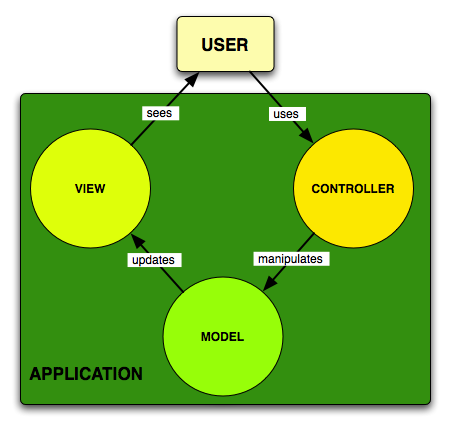
\includegraphics[width=0.5\textwidth]{reportCh2/mvc}
  \caption{MVC concept\cite{mvc_for_php}}
  \label{fig:mvc}
\end{figure}

PaWS is based on MVC\cite{mvc} design pattern. MVC stands for \emph{Model-View-Controller} and is an architectural design pattern for software engineering, especially for creating applications with graphical user interface. 

As can be seen on the figure \ref{fig:mvc}, MVC divides the application into three parts: 
\begin{itemize}
  \item {\bf Model}, which is the representation of problem or application logic, 
  \item {\bf View}, which describes how to display some parts of model in the user interface,
  \item {\bf Controller}, which is responsible for communication with user, like receiving input data or updating model and refreshing view in reaction to user actions.
\end{itemize}

In PaWS framework, the Model layer is not present, because there is no specific data logic and nor database is used. However, PaWS could be extended by adding for example user authentication or customization for users (like remembering preferences) and, in this case, a database (and Model layer) will be necessary.

\subsection{Architecture overview}

PaWS is a framework which shares its functionality remotely. 
\begin{figure}[h!]
  \centering
  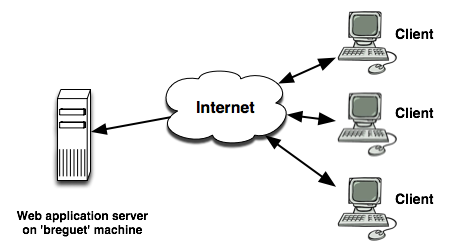
\includegraphics[width=0.5\textwidth]{reportCh2/web_applications}
  \caption{Architecture of access to web applications}
  \label{fig:web_applications}
\end{figure}
That means that there is no need of installing it on the machine of client and PaWS can be reached via the Internet as it is presented in the Figure \ref{fig:web_applications}. Clients need only a web browser - so called \emph{thin client}. A \emph{Thin client} can be a terminal or a computer. It needs another machine (its server) to perform its tasks. Advantages of this approach is lack of necessity to install special tools on client machines, independence from changes of software on the server and low load of the clients machine. Disadvantages of this solution may be: reduced functionality on the client side, requirement to establish internet connection to perform the tasks and all of the limitations resulting from the usage the network (latency, bandwidth).

In addition, in PaWS there is PIPS running, as it is presented on the figure \ref{fig:webapp_paws}. What is more, Pyrops (which is described in section \ref{other_technologies}) enables remote usage of PIPS and what follows, distribution of the application is case of load balancing.


\begin{figure}[h!]
  \centering
  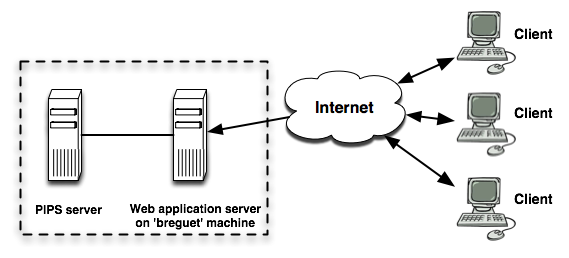
\includegraphics[width=0.5\textwidth]{reportCh2/webapp_paws}
  \caption{Architecture of access to PaWS}
  \label{fig:webapp_paws}
\end{figure}

PaWS architecture is not complicated and consists of 3 layers. It is presented in the Figure \ref{fig:paws_architecture}.

\begin{figure}[h!]
  \centering
  
\includegraphics[width=0.7\textwidth]{reportCh2/paws}
  \caption{Architecture of PaWS}
  \label{fig:paws_architecture}
\end{figure}

The top layer is {\bf PaWS web application}. It consists of:

\begin{itemize}
  \item {\bf HTML code} part, which is responsible for graphical user interface. It is equivalent of the 'View' layer in MVC. HTML sites are built on the basis of the relevant templates in the Mako language. Each PaWS mode (like tutorial, basic tools etc.) has separate templates for creating adequate site. Content of web pages is supplied by structure of files with descriptions (i.e. examples or PIPS basic tools). {\bf Ajax} part of this layer is responsible for the dynamic content of the site and for communication with controllers layer, i.e. for passing variables between those two layers.
  \item {\bf Pylons controllers} part, which is responsible for interception and interpretation of the user input. It also can pass output back to the view layer. Pylons controllers are a simple and powerful solution. They are special Python classes, which are very easy to customize. In PaWS, the controllers layer is also responsible for passing input and getting output of operations of lower layers.
\end{itemize}

The two lower layers are linked together very tightly. The middle layer is composed of three parts. The first of them, {\bf Pylons} is the core of web application and provides all web server functionalities described in section \ref{pylons_descriptions}. The other two parts: PyPS (see: \ref{pips_and_pyps}) and Tpips (see: \ref{tpips_interface}) are interfaces for PIPS framework.

The lowest layer is the kernel of the whole system and is composed of two parts:

\begin{itemize}
  \item {\bf Python} (described in \ref{python_description}), which is the base for Pylons and PyPS mechanisms.
  \item {\bf PIPS core} (described in \ref{pips_and_pyps}), which provides all of the transformations and analysis.
\end{itemize}

Middle layer with interfaces is necessary for proper activity of PaWS. Both Tpips and PyPS simplifies usage of PIPS and encapsulate its functionalities. What is more, due to PyPS it is easier to link Pylons Controllers with PIPS operations - it enables to invoke PIPS methods from Python code (directly in controller or by importing prepared modules).

\subsection{Structure}
\label{structure}

PaWS framework files and directories structure consists of two main parts: Pylons related and PIPS related.

\begin{figure}[h!]
  \centering
  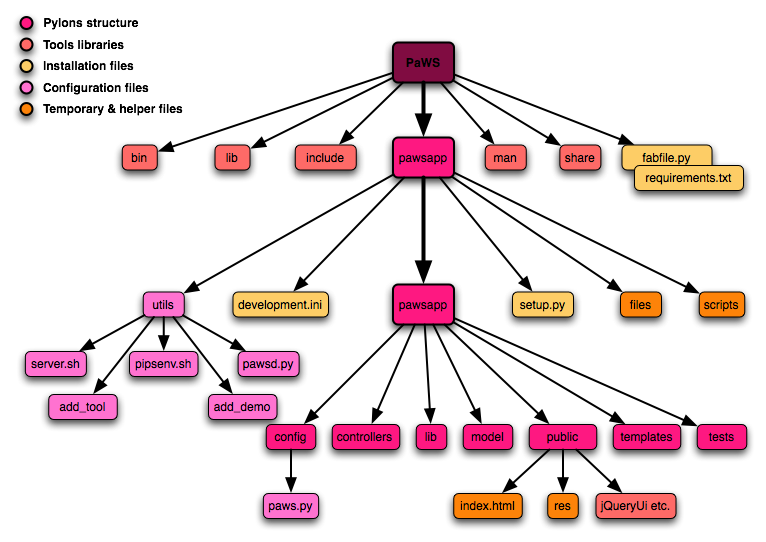
\includegraphics[width=1.0\textwidth]{reportCh2/paws-structure}
  \caption{File structure of PaWS}
  \label{fig:paws_structure}
\end{figure} 

The first one, shown in the Figure \ref{fig:paws_structure}, is based on Pylons project directories structure. Files and directories here can be classified into 5 types:
\begin{enumerate}
  \item {\bf The Pylons structure} directories which contain source code of PaWS framework. They are described in following section \ref{architecture_elements}.
  \item {\bf The installation files} - files used during the process of installation PaWS on user's machine. Two of them \emph{development.ini} and \emph{setup.py} refer to Pylons directly and can be also used as a configuration files. \emph{Fabfile.py} and \emph{requirements.txt} are the files of Fabric framework (see section \ref{other_technologies}) designed for quick installation of the all dependencies of PaWS framework. More details can be found in the section about PaWS installation \ref{installation}.
  \item {\bf The configuration files} - all of the files which can be modified by user to get the proper settings for his PaWS instance. To this group also scripts to manipulate the application content are belonging:
  \begin{itemize}
    \item {\bf add\_tool}: a script used to add a new analysis or transformation, described in the Section \ref{add_analysis_transformation}.
    \item {\bf add\_demo}: a script used to add a new demonstration, described in the section \ref{add_demonstration}.
    \item {\bf pipsenv.sh}: a script which is responsible for adding necessary directories to the path and system variables.
    \item {\bf pawsd.py}: a script which is responsible for deleting old temporary files.
    \item {\bf server.sh}: a script for starting application server.
  \end{itemize}
  \item {\bf Temporary and helper files} created by PaWS - directories and files which are necessary for PaWS work, but are not the part of Pylons architecure. They should not be changed by a user. Directories \emph{files} and \emph{res} are storing files temporary created during the PIPS operations, directory \emph{scripts} containts scripts related to adding new functionalities of PaWS and \emph{index.html} is responsible for redirectoring user to the PaWS introduction web page.
  \item {\bf Libraries} - directories and files of the tools which support work of PaWS, like VirtualEnv (described in \ref{virtualenv}) section or web applications technologies libraries (described in \ref{web_application_technologies} section).
\end{enumerate}

On the highest level there are mainly libraries and binaries related to the tools used by PaWS, i.e. Virtualenv described in \ref{virtualenv}.

The second part of PaWS structure used for configuration, presented in the Figure \ref{fig:pips_structure}, is located in the PIPS \emph{validation} directory and is mapping abstract PaWS division into modes, such as tutorial or full control (described in section \ref{paws_project}) onto the physical directories structure.

\begin{figure}[h!]
  \centering
  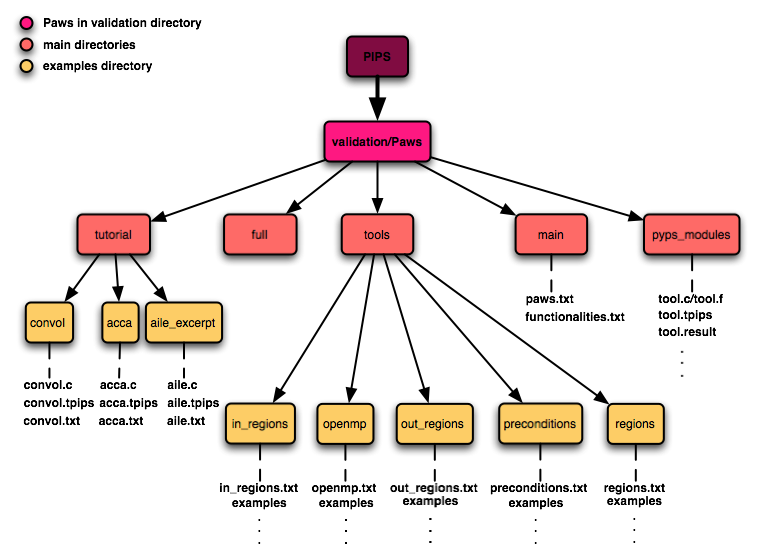
\includegraphics[width=1.0\textwidth]{reportCh2/pips-structure}
  \caption{Structure of PIPS part of PaWS}
  \label{fig:pips_structure}
\end{figure}

\subsection{Architecture elements}
\label{architecture_elements}

This section contains descriptions of the main types of PaWS framework elements: controllers, templates, validation directory and libraries.

\subsubsection{Controllers}

As it is described in the previous section, controllers are responsible for performing actions at the user request. In PaWS several types of controllers are used. 

\begin{enumerate}
  \item Controllers responsible for hosting web sites and contains only one method ``index''. They are created automatically when adding new functionality. Their names correspond to the functionality they respresent (i.e. ``tools preconditions'' or ``tutorial convol'')
  \item Controllers responsible for creating special web sites, like ``paas'' controller for introduction page or ``descriptions'' controller for extracting information from the structure of description files.
  \item Controllers responsible for linkage with PyPS or Tpips for performing operations. There are three controllers this type: ``operations'' for basic tools (both basic and advanced level), ``demo'' for tutorial and ``graph'' for creating dependence graps.
  \item Controllers for other operations which are not using PIPS. To this group belong controller ``detector'' responsible for detecting language of source code and ``examples'' controller which is loading supplied examples.
\end{enumerate}

\subsubsection{Templates}

Templates are the files which provide code for web sites. They are a very convenient solution because they allow to combine HTML, Javascript and Python code. What is more, especially when web application consists of many similar pages, templates technology allows to use the inheritance between templates. That significantly reduces the amount of redundant code. 

PaWS consist of several types of templates:

\begin{itemize}
  \item ``Skeleton'' templates, which provide necessary (and common for all of the pages) operations for application to work (like uploading files, changing font size or checking if the input source code is correct). Those templates (like ``frame'' template) are creating structures which are inherited by other, more specific, templates.
  \item Templates which are creating frame code dedicated to the specific PaWS mode (like tutorial, basic PIPS tools or advanced PIPS tools). They are inheriting from more general skeleton templates. 
  \item Templates which are responsible for creating specific web site dedicated to the special case (one tutorial or PIPS tool). Each of them inherits from the appropriate mode template and provides characteristic information, such as the name of the PIPS tool or the name of tutorial file.
  \item ``Paas'' template which is responsible for introduction page, and for extracting information about available tools from the description files.
\end{itemize}

\subsubsection{Other modules}
\label{other_modules}

PaWS consists also of some other modules:

\begin{itemize}
  \item {\bf \emph{validation}} is the directory of PIPS project where all the supplied examples are placed. All of the samples each day undergo validation. PaWS validation directory is placed in PIPS repository in \emph{validation/Paws} and consists of several directories:
  \begin{itemize}
    \item {\bf \emph{pyps\_modules}} described below;
    \item {\bf \emph{tutorial}} which contains all of the demonstration examples;
    \item {\bf \emph{tools}} which contains subdirectories with examples dedicated to concrete tool (like \emph{preconditions} or \emph{openmp}). Those directories are named after mode they refer to;
  \end{itemize}
  \item {\bf PyPS modules} are the part of \emph{validation} directory (named \emph{pyps\_modules}). Each module contains PyPS code necessary to perform some analysis or transformation. As all of the cases kept in \emph{validation} directory because those modules also should undergo validation each day.
  \item {\bf \emph{public}} is the Pylons directory where all of the helper but not directly connected to the Pylons or PIPS tools and features are placed. In example, all of the Javascript libraries, images used by PaWS or description files are stored here. 
  \item {\bf \emph{lib}} is the Pylons directory for all of the helper Python libraries and modules used by PaWS (like base Pylons controller, helper for managing files or detectors of programming languages).
  \item {\bf \emph{tests}} is the Pylons directory for functional tests for controllers.
\end{itemize}

\subsection{Flows and scenarios}

This section shows how different elements of PaWS architecture are linked together. Basic flows for each mode are presented and described here. Each mode has several cases, different tools or different demo examples, but in each case the scenario of operation performed remains the same.

\begin{figure}[h!]
  \centering
  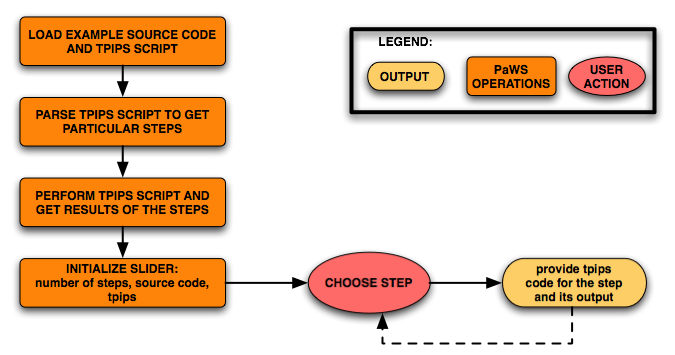
\includegraphics[width=0.7\textwidth]{reportCh2/tutorial_flow}
  \caption{Tutorial flow mode}
  \label{fig:tutorial_flow}
\end{figure}

\begin{itemize}
  \item {\bf Demo mode}: there are three scenarios available: \emph{aile\_excerpt}, \emph{convol} and \emph{acca-2011}. Input and all of the possible operations and their sequence are provided by the application - user only controls the step. The basic flow is presented on the Picture \ref{fig:tutorial_flow}.
  
  \begin{figure}[h!]
  \centering
  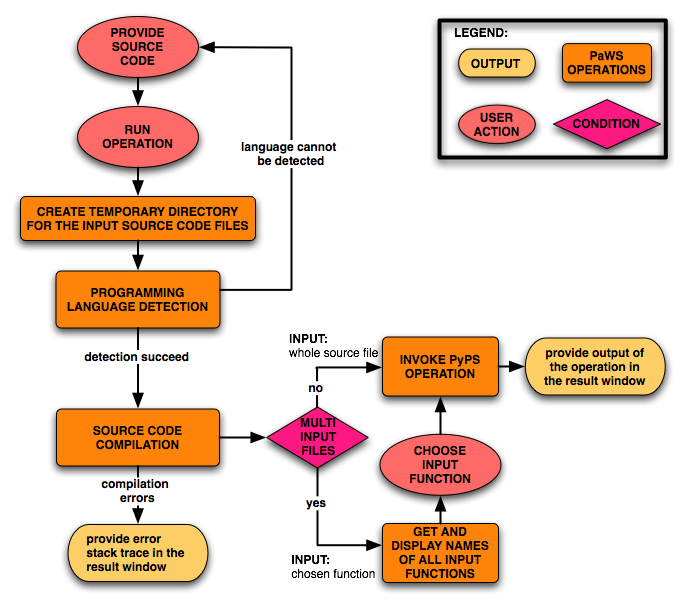
\includegraphics[width=0.7\textwidth]{reportCh2/basic_tool_flow}
  \caption{Basic tool flow mode}
  \label{fig:basic_tool_flow}
\end{figure}

\begin{figure}[h!]
  \centering
  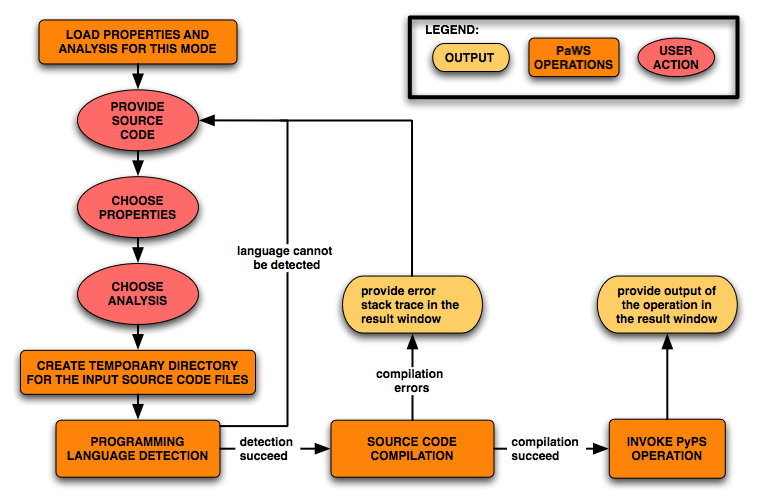
\includegraphics[width=0.7\textwidth]{reportCh2/advanced_tool_flow}
  \caption{Advanced tool flow}
  \label{fig:advanced_tool_flow}
\end{figure}
  
  \item {\bf Basic tools - basic level}: five tools are currently configured: \emph{preconditions}, \emph{IN regions}, \emph{OUT regions}, \emph{regions} and \emph{OpenMP}. This PaWS mode allows user to either choose one of supplied examples, different for each type of tools, or to provide input source code by him/herself (by uploading file or by directly typing or cut-and-pasting in application window). The basic flow of this mode is shown in the Picture \ref{fig:basic_tool_flow}.

  \item {\bf Basic tools - advanced level}: there are two tools available: \emph{preconditions} and \emph{regions}. This mode is similar to the basic level - source code can be provided in the same way here. Basic scenario is displayed on the picture \ref{fig:advanced_tool_flow}.
  
  \item {\bf Full control}: NOT DEVELOPED
  There was not enough time.
\end{itemize}